%----------------------------------------------------------------------------------------
%	PACKAGES AND OTHER DOCUMENT CONFIGURATIONS
%----------------------------------------------------------------------------------------

\documentclass[12pt]{article}
\usepackage[english]{babel}
\usepackage[utf8x]{inputenc}
\usepackage{amsmath}
\usepackage{graphicx}
\usepackage{float}
\usepackage[colorinlistoftodos]{todonotes}
\usepackage{efbox,graphicx}
\efboxsetup{linecolor=black,linewidth=1pt}
\usepackage{natbib}
\usepackage{hyperref}
\usepackage{caption}
\usepackage{caption,float}
\usepackage[vmargin=3cm,hmargin=3cm]{geometry}

\begin{document}

\begin{titlepage}

\newcommand{\HRule}{\rule{\linewidth}{0.5mm}} % Defines a new command for the horizontal lines, change thickness here

\center % Center everything on the page
 
%----------------------------------------------------------------------------------------
%	HEADING SECTIONS
%----------------------------------------------------------------------------------------

\textsc{ Memorial University of Newfoundland}\\[1.5cm] % Name of your university/college

\includegraphics[scale=.1]{MUN_Logo.jpg}\\[1cm] % Include a department/university logo - this will require the graphicx package
\textsc{\Large Computer Based Research Tools and Applications}\\[0.5cm] % Major heading such as course name
\textsc{\large CMSC6950}\\[0.5cm] % Minor heading such as course title

%----------------------------------------------------------------------------------------
%	TITLE SECTION
%----------------------------------------------------------------------------------------

\HRule \\[0.4cm]
{ \huge \bfseries RADWave: Python code for ocean surface wave analysis by satellite radar altimeter}\\[0.4cm] % Title of your document
\HRule \\[1.5cm]
 
%----------------------------------------------------------------------------------------
%	AUTHOR SECTION
%----------------------------------------------------------------------------------------

% If you don't want a supervisor, uncomment the two lines below and remove the section above
\Large \emph{Author:}\\
Soheil Mousavi Moghaddam\\[3cm] % Your name

%----------------------------------------------------------------------------------------
%	DATE SECTION
%----------------------------------------------------------------------------------------

{\large August, 2020}\\[2cm] % Date, change the \today to a set date if you want to be precise

\vfill % Fill the rest of the page with whitespace

\end{titlepage}

\newpage

{
  \section*{Abstract}
}
RADWave allows the user to query over a range of spatial and temporal scales altimeter parameters in specific geographical regions and subsequently calculates significant wave heights, periods, group velocities, average wave energy densities and wave energy fluxes. In the following we are going to test some of these features on our dataset \\\\

\section{Our Data}
\subsection{Introduction}
The AODN (Australian Ocean Data Network) provides access to all available Australian marine and climate science data and provides the primary access to IMOS (Integrated Marine Observing System) data including access to the IMOS metadata. With the help of this data and by using RADWave module on python, we can make plots to observe wave conditions based on altimeter data for a specific geographical region over a period of time.
\subsection{The Dataset}
Our dataset (altimeterData.csv) has 5 columns and 13670 rows. In addition we use a text file (IMOSURLs.txt) which consist of a list of URLs that help us communicate to satellites for our desired time period and geographical region. Below is a description of each column in the altimeterData.csv: 

\begin{itemize}

\item lon: Longitude, is a geographic coordinate that specifies the east–west position of a point on the Earth's surface
\item lat: Latitude, is a geographic coordinate that specifies the north–south position of a point on the Earth's surface
\item wh: Wave Height, the height that the wave achieved in meters 
\item time: Time of the occurrence of the wave
\item ws: Wave Second, the period that took for the wave to happen in seconds

\end{itemize}

\newpage
\section{Workflow Analysis}
\subsection{Processing altimeters data}
Here we use RADWave to extract wave conditions based on altimeter data for a specific geographical region. At first we need to find our desired geographical location. My chosen dataset is for a region of the see at the west coast of Sydney. On the dataset there is the data regarding to recording of wave movements over the period form January of 1995 until January of 2020. Using \texttt{waveAnalysis.visualiseData} we can create a figure with the location of our wave recordings on a map.\figureautorefname{1}

\begin{figure}[h]
    \centering
    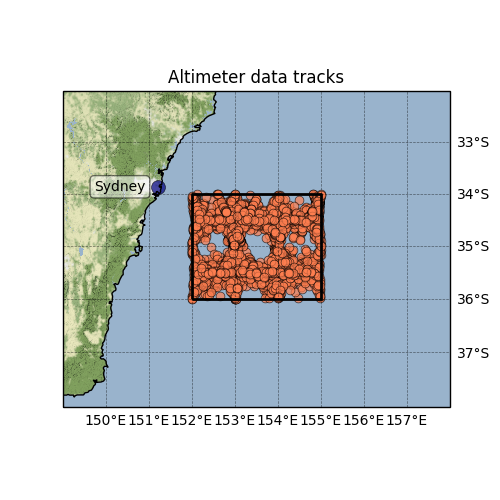
\includegraphics[width=8 cm]{altimeterdata.png}
    \caption{a nice plot}
    \label{fig:fig1}
\end{figure}

\subsection{Computing wave regime}
Based on our data, to perform wave analysis and compute the wave parameters, we run the \texttt{generateTimeSeries} function. This function computes time series of wave characteristics from available altimeter data namely the significant wave height and the wind speed. It computes both \textbf{instantaneous} and \textbf{monthly} wave variables and saves it as a Pandas dataframe. We can now plot time series of RADWave calculated wave parameters by calling \texttt{plotTimeSeries} function.
\figureautorefname{2} and \figureautorefname{3} show the maximum and minimum size of wave heights and power with the monthly average over the span of 25 years. Also by using the data in our dataframe we can create a scatter plot using the longitude and latitude of waves and coloring them regarding their energy level (\figureautorefname{4}).
\newpage

\begin{figure}[h]
    \centering
    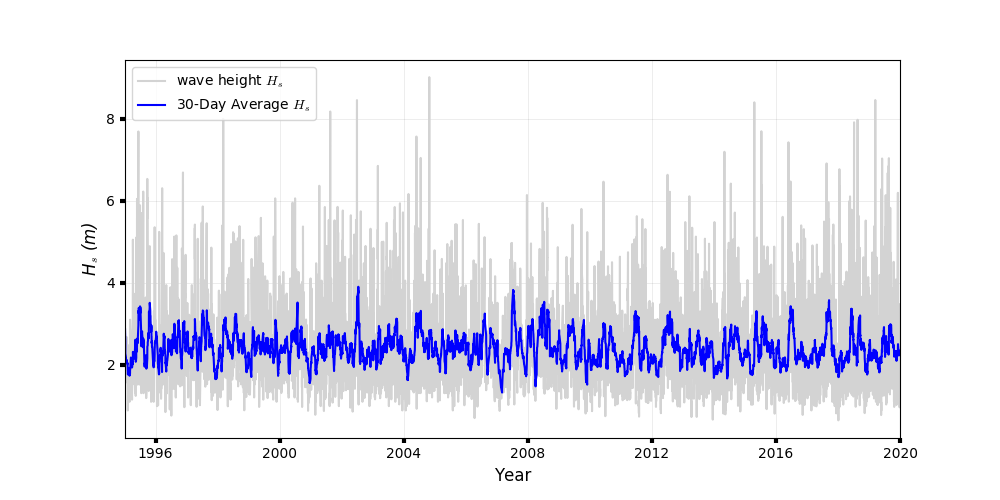
\includegraphics[width=12 cm]{Hseries.png}
    \caption{Waves Height}
    \label{fig:fig2}
\end{figure}

\begin{figure}[h]
    \centering
    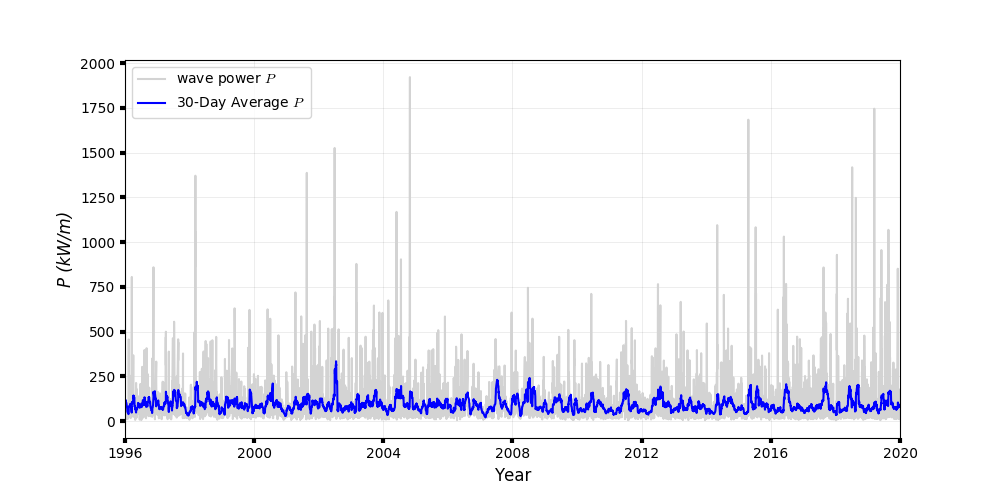
\includegraphics[width=12 cm]{Pseries.png}
    \caption{Waves Power}
    \label{fig:fig3}
\end{figure}

%\begin{figure}[h]
%    \centering
%    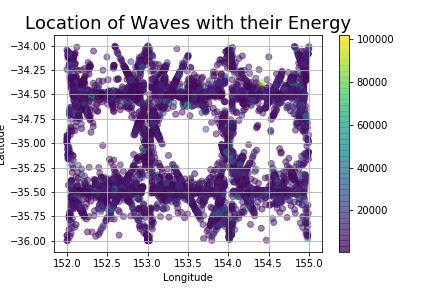
\includegraphics[width=8 cm]{wave_location.png}
%    \caption{}
%    \label{fig:fig4}
%\end{figure}

\newpage

\subsection{Processing wave seasonal trends}
in addition to time series, we can analyse the seasonal characteristics of each parameter computed from the altimeter dataset.We used this to draw a heat map of the significant wave heights in each month over the past 25 years (\figureautorefname{5}). And we can see the distribution of this heat-map that can help us better identify which months have higher wave heights (\figureautorefname{6}). 

\begin{figure}[h]
    \centering
    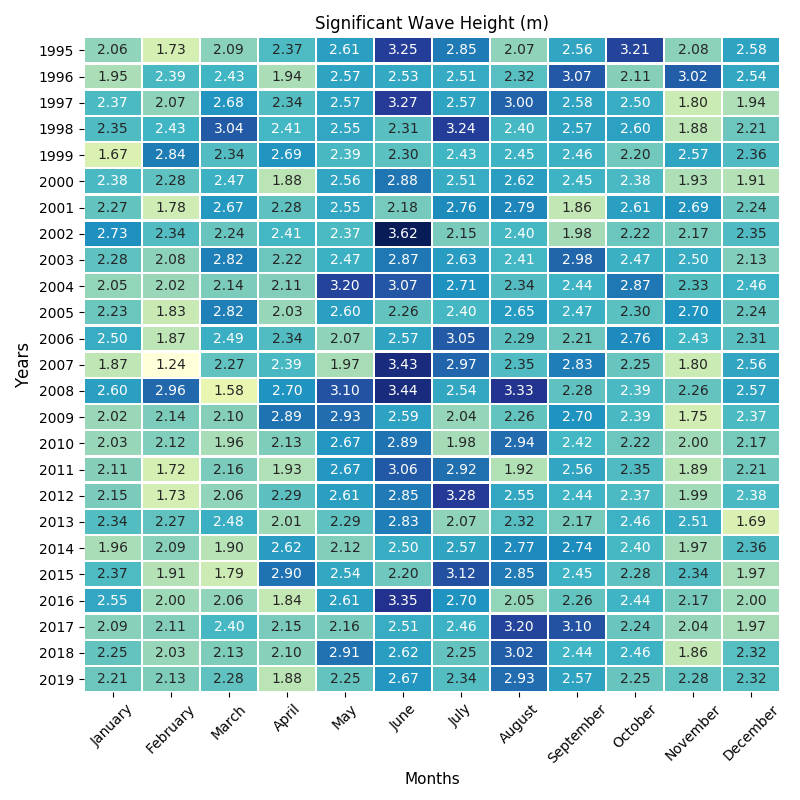
\includegraphics[width=10 cm]{whall_wh_heatmap.png}
    \caption{Heat-map of significant wave heights}
    \label{fig:fig5}
\end{figure}

\begin{figure}[h]
    \centering
    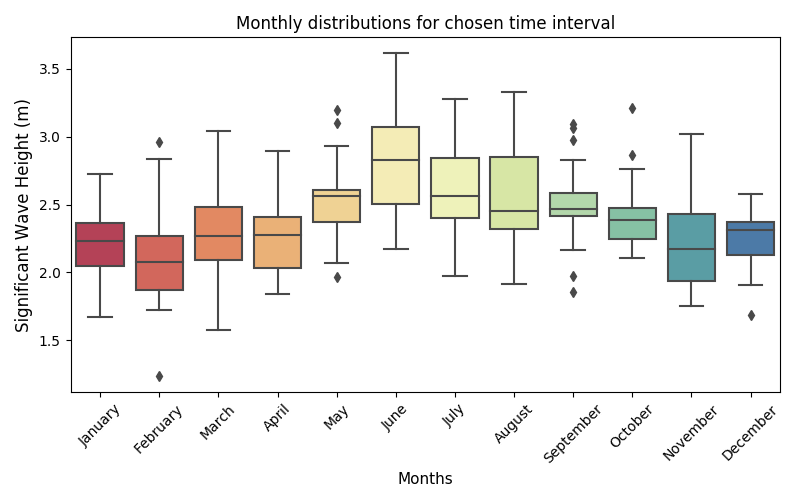
\includegraphics[width=6.5 cm]{whall_wh_distribution.png}
    \caption{Heat-map of significant wave heights}
    \label{fig:fig6}
\end{figure}

\newpage

\subsection{Annual values for each tile}
The data we have of the ocean are put in our dataset as a series of tiles that cover the oceans. Each tile has its individual longitude and latitude. We can make annual reports for each tile and based on the mean of their monthly, seasonally or annual activities (\figureautorefname{7}). 

\begin{figure}[h]
    \centering
    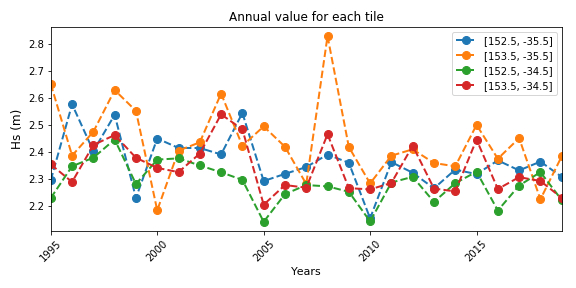
\includegraphics[width=12 cm]{annual_value.png}
    \caption{Heat-map of significant wave heights}
    \label{fig:fig7}
\end{figure}
 Here we can observe that each color represent changes in annual mean value of wave heights for each one of the four tiles that I chose to show.
 
\section{Conclusion}
Overall, in my opinion RADWave is a very strong package in this field and what we saw here was only a small portion of the  things that can be done using this package. It has a easy to use syntax and a complete documentation to help you with it. It is also should be noted that most of the data available to use are for the regions and oceans near Australia and that can be problematic if you are looking to analyze another part of the world. 
\newline In this project we observed some figures on the ocean waves and specially the height of the wave over the period of past 25 years and it can give us some ideas regarding which seasons or which years had a calmer ocean surface and which years went to the extremes in the records.
\newpage

\begin{thebibliography}{9}

    \bibitem{ref1}
    Courtney Smith and Tristan Salles and Ana Vila-Concejo | RADWave: Python code for ocean surface wave analysis by     satellite radar altimete. Retrieved from Journal of Open Source Software 
    {\url{https://doi.org/10.21105/joss.02083}}
   
	\bibitem{ref2}
	Integrated Marine Observing System (IMOS), Australia
	{\url{http://imos.org.au/}}
	

	\bibitem{ref3}
	Australian Ocean Data Network (AODN), Australia
	{\url{https://portal.aodn.org.au/}}


\end{thebibliography}

\end{document}